% Created by tikzDevice version 0.7.0 on 2015-04-20 21:47:30
% !TEX encoding = UTF-8 Unicode
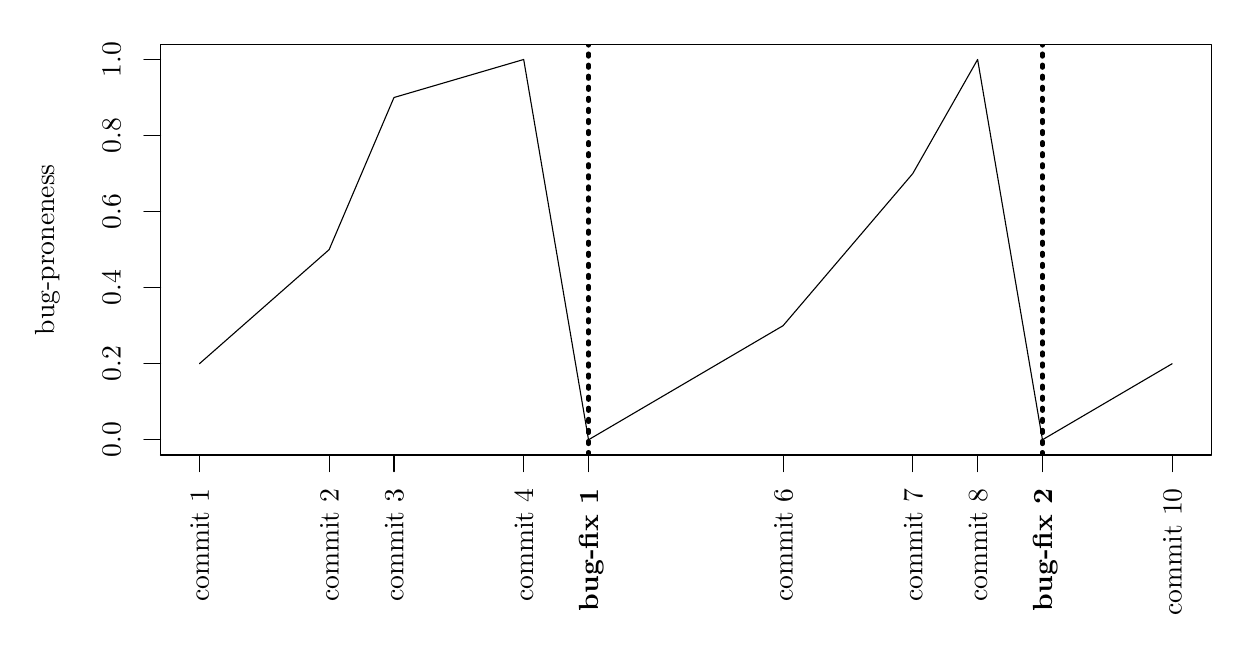
\begin{tikzpicture}[x=1pt,y=1pt]
\definecolor[named]{fillColor}{rgb}{1.00,1.00,1.00}
\path[use as bounding box,fill=fillColor,fill opacity=0.00] (0,0) rectangle (433.62,216.81);
\begin{scope}
\path[clip] ( 48.00, 62.40) rectangle (427.62,210.81);
\definecolor[named]{drawColor}{rgb}{0.00,0.00,0.00}

\path[draw=drawColor,line width= 0.4pt,line join=round,line cap=round] ( 62.06, 95.38) --
	(108.93,136.60) --
	(132.36,191.57) --
	(179.23,205.31) --
	(202.66, 67.90) --
	(272.96,109.12) --
	(319.83,164.09) --
	(343.26,205.31) --
	(366.69, 67.90) --
	(413.56, 95.38);
\end{scope}
\begin{scope}
\path[clip] (  0.00,  0.00) rectangle (433.62,216.81);
\definecolor[named]{drawColor}{rgb}{0.00,0.00,0.00}

\path[draw=drawColor,line width= 0.4pt,line join=round,line cap=round] ( 48.00, 67.90) -- ( 48.00,205.31);

\path[draw=drawColor,line width= 0.4pt,line join=round,line cap=round] ( 48.00, 67.90) -- ( 42.00, 67.90);

\path[draw=drawColor,line width= 0.4pt,line join=round,line cap=round] ( 48.00, 95.38) -- ( 42.00, 95.38);

\path[draw=drawColor,line width= 0.4pt,line join=round,line cap=round] ( 48.00,122.86) -- ( 42.00,122.86);

\path[draw=drawColor,line width= 0.4pt,line join=round,line cap=round] ( 48.00,150.35) -- ( 42.00,150.35);

\path[draw=drawColor,line width= 0.4pt,line join=round,line cap=round] ( 48.00,177.83) -- ( 42.00,177.83);

\path[draw=drawColor,line width= 0.4pt,line join=round,line cap=round] ( 48.00,205.31) -- ( 42.00,205.31);

\node[text=drawColor,rotate= 90.00,anchor=base,inner sep=0pt, outer sep=0pt, scale=  1.00] at ( 33.60, 67.90) {0.0};

\node[text=drawColor,rotate= 90.00,anchor=base,inner sep=0pt, outer sep=0pt, scale=  1.00] at ( 33.60, 95.38) {0.2};

\node[text=drawColor,rotate= 90.00,anchor=base,inner sep=0pt, outer sep=0pt, scale=  1.00] at ( 33.60,122.86) {0.4};

\node[text=drawColor,rotate= 90.00,anchor=base,inner sep=0pt, outer sep=0pt, scale=  1.00] at ( 33.60,150.35) {0.6};

\node[text=drawColor,rotate= 90.00,anchor=base,inner sep=0pt, outer sep=0pt, scale=  1.00] at ( 33.60,177.83) {0.8};

\node[text=drawColor,rotate= 90.00,anchor=base,inner sep=0pt, outer sep=0pt, scale=  1.00] at ( 33.60,205.31) {1.0};

\path[draw=drawColor,line width= 0.4pt,line join=round,line cap=round] ( 48.00, 62.40) --
	(427.62, 62.40) --
	(427.62,210.81) --
	( 48.00,210.81) --
	( 48.00, 62.40);
\end{scope}
\begin{scope}
\path[clip] (  0.00,  0.00) rectangle (433.62,216.81);
\definecolor[named]{drawColor}{rgb}{0.00,0.00,0.00}

\node[text=drawColor,rotate= 90.00,anchor=base,inner sep=0pt, outer sep=0pt, scale=  1.00] at (  9.60,136.60) {bug-proneness};
\end{scope}
\begin{scope}
\path[clip] (  0.00,  0.00) rectangle (433.62,216.81);
\definecolor[named]{drawColor}{rgb}{0.00,0.00,0.00}

\path[draw=drawColor,line width= 0.4pt,line join=round,line cap=round] ( 62.06, 62.40) -- (413.56, 62.40);

\path[draw=drawColor,line width= 0.4pt,line join=round,line cap=round] ( 62.06, 62.40) -- ( 62.06, 56.40);

\path[draw=drawColor,line width= 0.4pt,line join=round,line cap=round] (108.93, 62.40) -- (108.93, 56.40);

\path[draw=drawColor,line width= 0.4pt,line join=round,line cap=round] (132.36, 62.40) -- (132.36, 56.40);

\path[draw=drawColor,line width= 0.4pt,line join=round,line cap=round] (179.23, 62.40) -- (179.23, 56.40);

\path[draw=drawColor,line width= 0.4pt,line join=round,line cap=round] (202.66, 62.40) -- (202.66, 56.40);

\path[draw=drawColor,line width= 0.4pt,line join=round,line cap=round] (272.96, 62.40) -- (272.96, 56.40);

\path[draw=drawColor,line width= 0.4pt,line join=round,line cap=round] (319.83, 62.40) -- (319.83, 56.40);

\path[draw=drawColor,line width= 0.4pt,line join=round,line cap=round] (343.26, 62.40) -- (343.26, 56.40);

\path[draw=drawColor,line width= 0.4pt,line join=round,line cap=round] (366.69, 62.40) -- (366.69, 56.40);

\path[draw=drawColor,line width= 0.4pt,line join=round,line cap=round] (413.56, 62.40) -- (413.56, 56.40);

\node[text=drawColor,rotate= 90.00,anchor=base east,inner sep=0pt, outer sep=0pt, scale=  1.00] at ( 65.50, 50.40) {commit 1};

\node[text=drawColor,rotate= 90.00,anchor=base east,inner sep=0pt, outer sep=0pt, scale=  1.00] at (112.37, 50.40) {commit 2};

\node[text=drawColor,rotate= 90.00,anchor=base east,inner sep=0pt, outer sep=0pt, scale=  1.00] at (135.80, 50.40) {commit 3};

\node[text=drawColor,rotate= 90.00,anchor=base east,inner sep=0pt, outer sep=0pt, scale=  1.00] at (182.67, 50.40) {commit 4};

\node[text=drawColor,rotate= 90.00,anchor=base east,inner sep=0pt, outer sep=0pt, scale=  1.00] at (206.10, 50.40) {\textbf{bug-fix 1}};

\node[text=drawColor,rotate= 90.00,anchor=base east,inner sep=0pt, outer sep=0pt, scale=  1.00] at (276.40, 50.40) {commit 6};

\node[text=drawColor,rotate= 90.00,anchor=base east,inner sep=0pt, outer sep=0pt, scale=  1.00] at (323.27, 50.40) {commit 7};

\node[text=drawColor,rotate= 90.00,anchor=base east,inner sep=0pt, outer sep=0pt, scale=  1.00] at (346.70, 50.40) {commit 8};

\node[text=drawColor,rotate= 90.00,anchor=base east,inner sep=0pt, outer sep=0pt, scale=  1.00] at (370.14, 50.40) {\textbf{bug-fix 2}};

\node[text=drawColor,rotate= 90.00,anchor=base east,inner sep=0pt, outer sep=0pt, scale=  1.00] at (417.00, 50.40) {commit 10};
\end{scope}
\begin{scope}
\path[clip] ( 48.00, 62.40) rectangle (427.62,210.81);
\definecolor[named]{drawColor}{rgb}{0.00,0.00,0.00}

\path[draw=drawColor,line width= 1.6pt,dash pattern=on 1pt off 3pt ,line join=round,line cap=round] (202.66, 62.40) -- (202.66,210.81);

\path[draw=drawColor,line width= 1.6pt,dash pattern=on 1pt off 3pt ,line join=round,line cap=round] (366.69, 62.40) -- (366.69,210.81);
\end{scope}
\end{tikzpicture}
